\documentclass[12pt,a4paper]{scrartcl}
\usepackage[utf8]{inputenc}
\usepackage[english,russian]{babel}
\usepackage{indentfirst}
\usepackage{misccorr}
\usepackage{graphicx}
\DeclareGraphicsExtensions{.pdf,.png,.jpg}
\graphicspath{{/}}
\usepackage{amsmath}

\begin{document}

\begin{center}
\begin{large}
Проект Кока-Кола
\end{large}
	\bigskip
     
Ахундзянов Амир Андреевич\\
Шуббе Леонтий Павлович
\end{center}

\section{Задачи и цели}
В ходе данного проекта планируется придумать методы для высокоточного сбора информации о состоянии жидкости  содержащей угольную кислоту и газа, находящихся и изолированном сосуде. После получения такой установки можно привести первичный анализ полученных данных и понять что-нибудь интересное про процесс выхода большого количества газа при встряске. Например можно проверить утверждение одного известного научного популяризатора. Он сказал, что после встряхивания бутылки с газировкой можно постучать по её стенкам для удаления маленьких пузырьков, которые увеличивают площадь поверхности жидкости, что ускоряет процесс выхода газа.

\section{Теоретическое обоснование}



\section{Методика и процесс создания оборудования}
Первоначально планировалось использовать механический манометр со стрелкой для измерения давления внутри бутылки с кока-колой и по диапазону измерений нам идеально подходил автомобильный манометр,\\
\begin{flushleft}
\includegraphics[scale=0.18]{Evalution}
\end{flushleft}

 но его использование вело к усложнению процесса сбора данных, так как значения приходилось снимать вручную, а изучемый процесс выхода газов мог идти около двух суток. Также точность измерения такого манометра далека от идеала. По этим и другим причинам было решено использовать электронный датчик давления MPXHZ6400AC6T1 , подключенный к микроконтроллеру Arduino Uno. Это позволило снимать показания без непосредственного участия человека и снизить погрешность до порядка 500 Паскалей. Таким образом, вклеив датчик в стандартную крышку для пластиковых бутылок, спаяв схему и написав прошивку для микроконтроллера мы собрали установку, измеряющую зависимость давления от времени.

Далее хотелось проводить такое исследование при постоянных, но разных температурах. Для охлаждения системы требуется сложное специализированное оборудование, поэтому мы удовлетворились одним измерением в холодильнике. Повышать же температуру много проще. Достаточно использовать простой нагреватель, как, наример, кипятильник. Поэтому следующим дополнением установки было подключение к Arduino реле, замыкающего питание нагревателя, опущенного в кастрюлю с водой, в которой лежала исследуемая бутылка. Для поддержания постоянства температуры воды вне занисимости от внешних условий был использован электронный датчик температуры DS18B20 в герметичном корпусе. 
\begin{flushleft}
\includegraphics[scale=0.16]{Heat}
\end{flushleft}

Еще одним параметром, который представлял для нас интерес, было количество вышедшего из раствора газа. Приборы измеряющие поток газа плохо подходили для наших целей, так как плохо работают с малыми скоростями выхода газа. Поэтому лучшим вариантом по нашему мнению было использовать излюбленный химиками способ сбора газов с помощью перевернутой в жидкость колбы. То есть мы взяли большую мензурку, так как в пол-литровой бутылке содержится более литра газа, и котел с водой. На дно мензурки прикрепляется один конец трубки из набор для капельницы и горлышко сосуда опускается под воду. Далее весь концентрированный $CO_2$ с прошлого эксперимента вытягивается из полости разумеется легкими и трубка перекрывается идущим в комплекте зажимом. Второй конец герметично вклеивается в крышку, которая надевается на бутылку с раствором. После открытия клапана можно снимать зависимость вышедшего газа от времени или просто количество газа, которое выходит при таком способе проведения измерения.
\begin{flushleft}
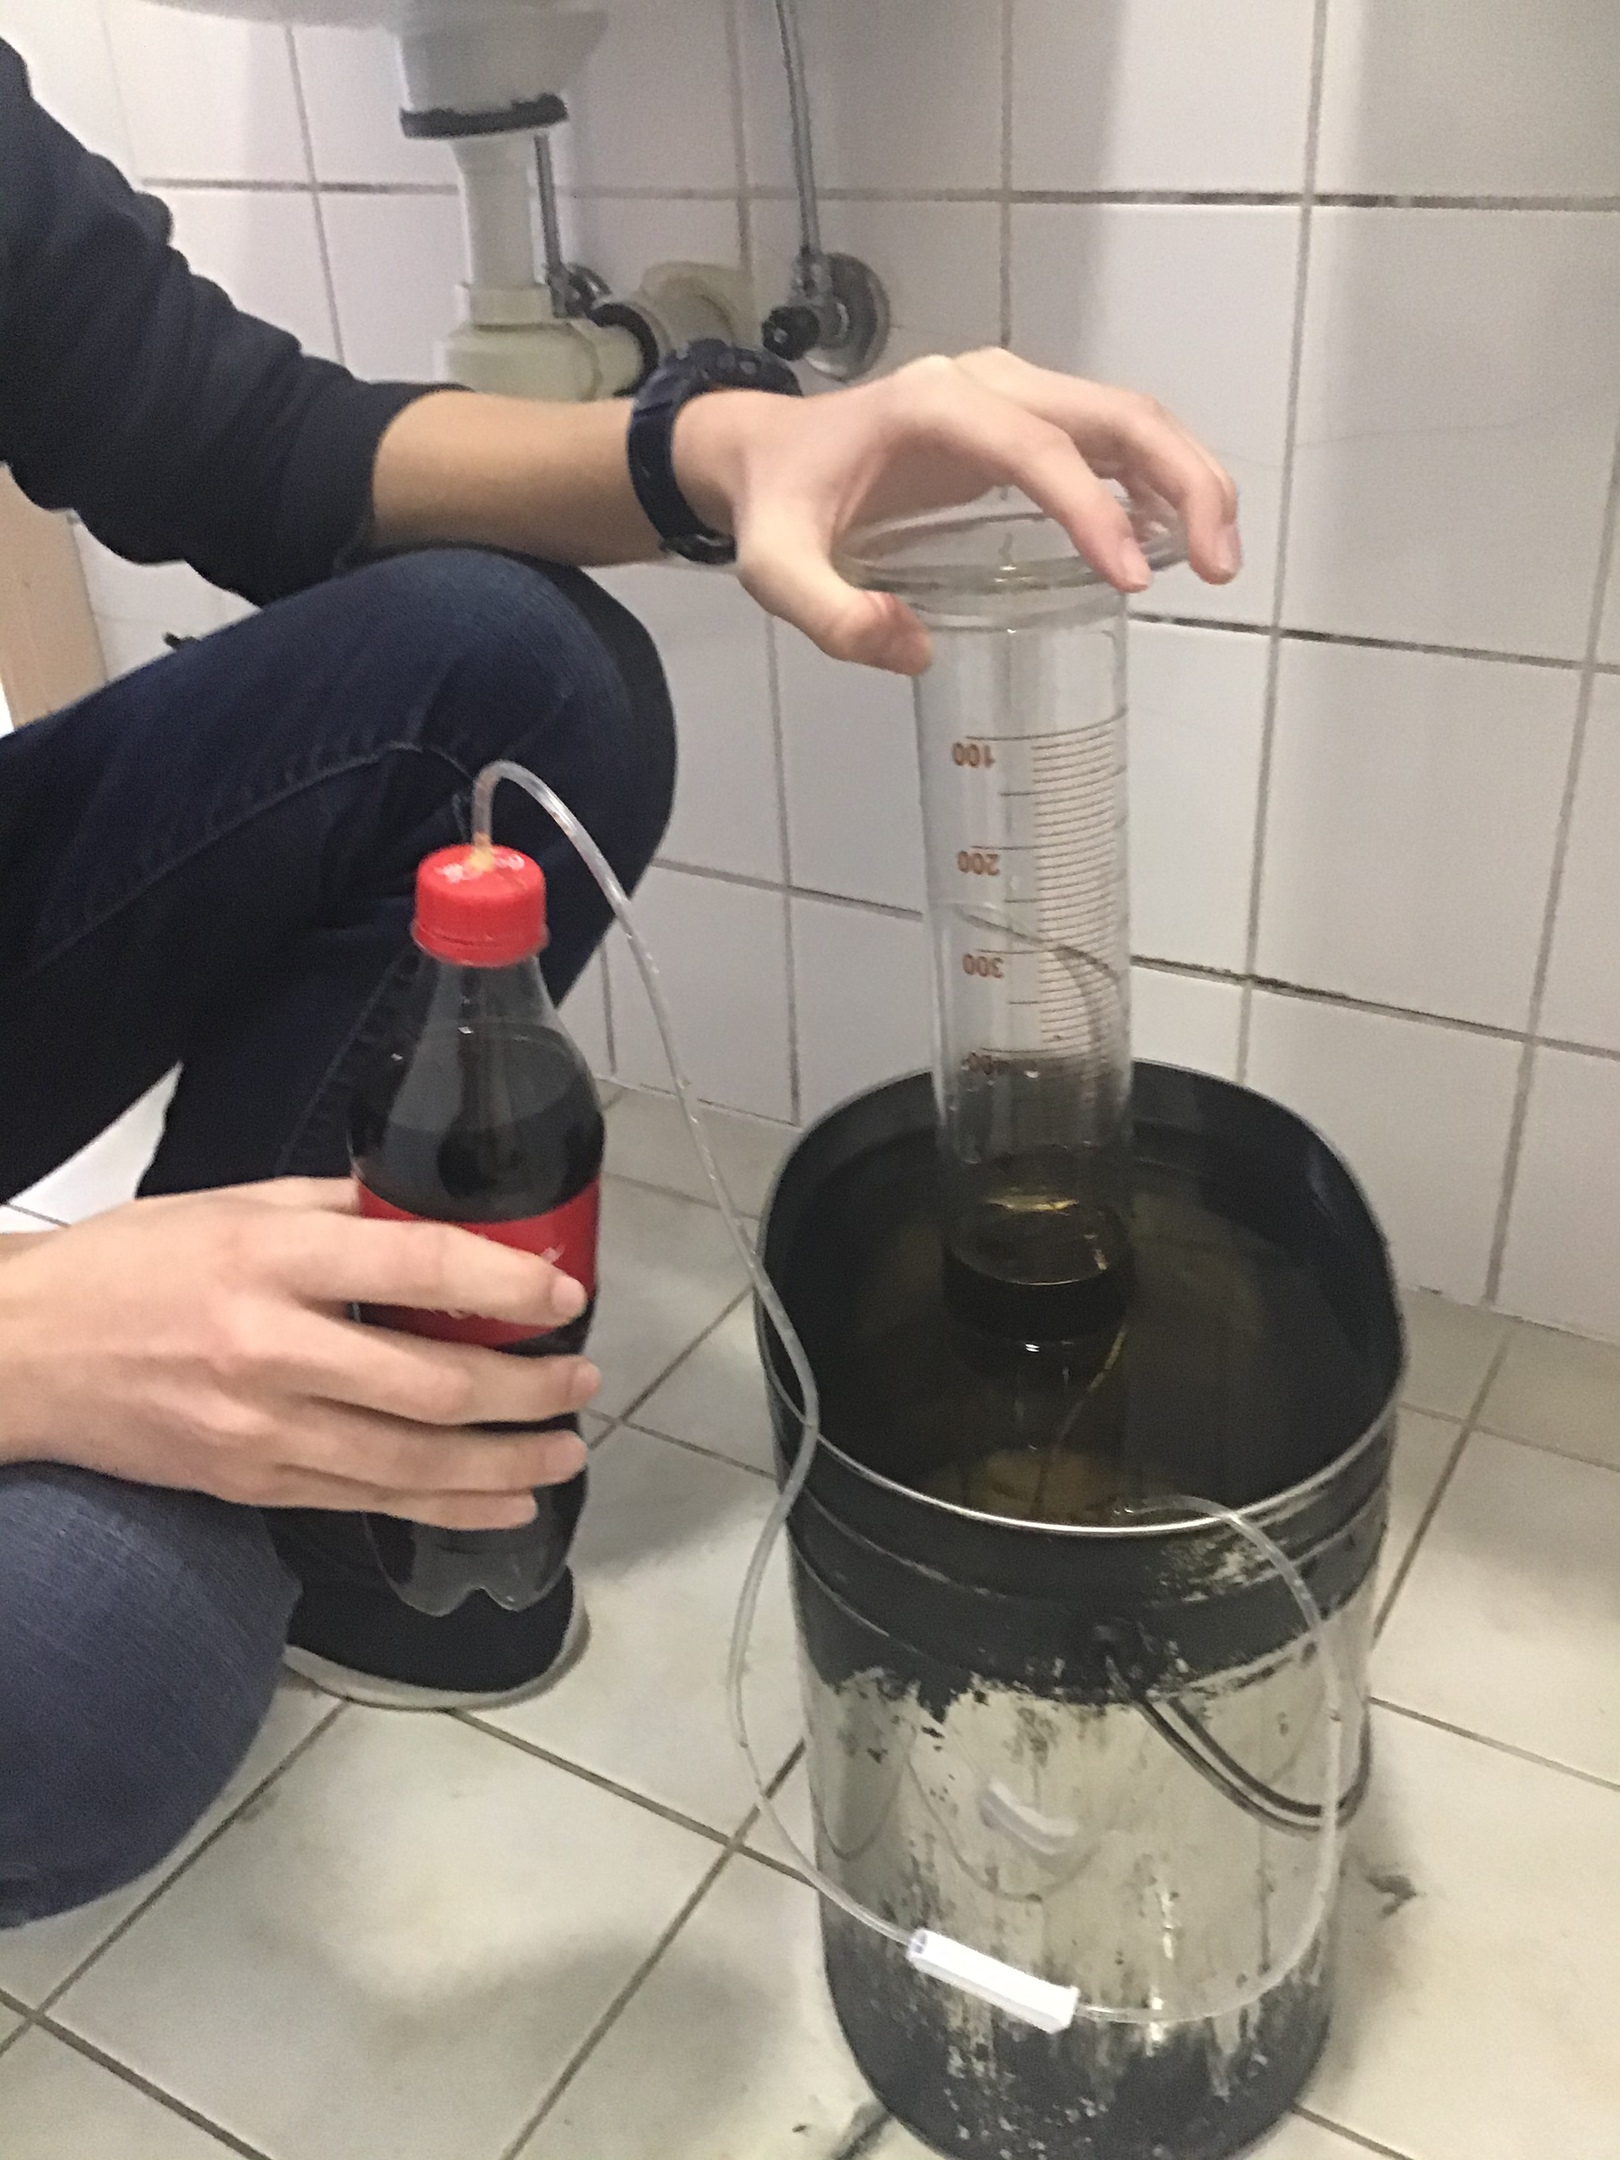
\includegraphics[scale=0.1]{ToiletFun}
\end{flushleft}
Чтобы измерить объем газа в бутылке пустая бутлка сначала была зополнена водой до того же уровня, что и неоткрытая бутылка и взвешена. После доливания воды до краев взвешивание повторили и по разнице масс и плотности воды был найден объем.

Штангенцирулем был измерен диаметр круговой поверхности жидкости и из этого была вычислена площдь поверхности.

\section{Результаты измерений и обработка данных}
Были провведены измерения зависимостей давления от времени при разных температурах и они хорошо описывались теоретической зависимостью $ p(t) = a - b\cdot e^{-\frac{t}{c}}$
\begin{flushleft}
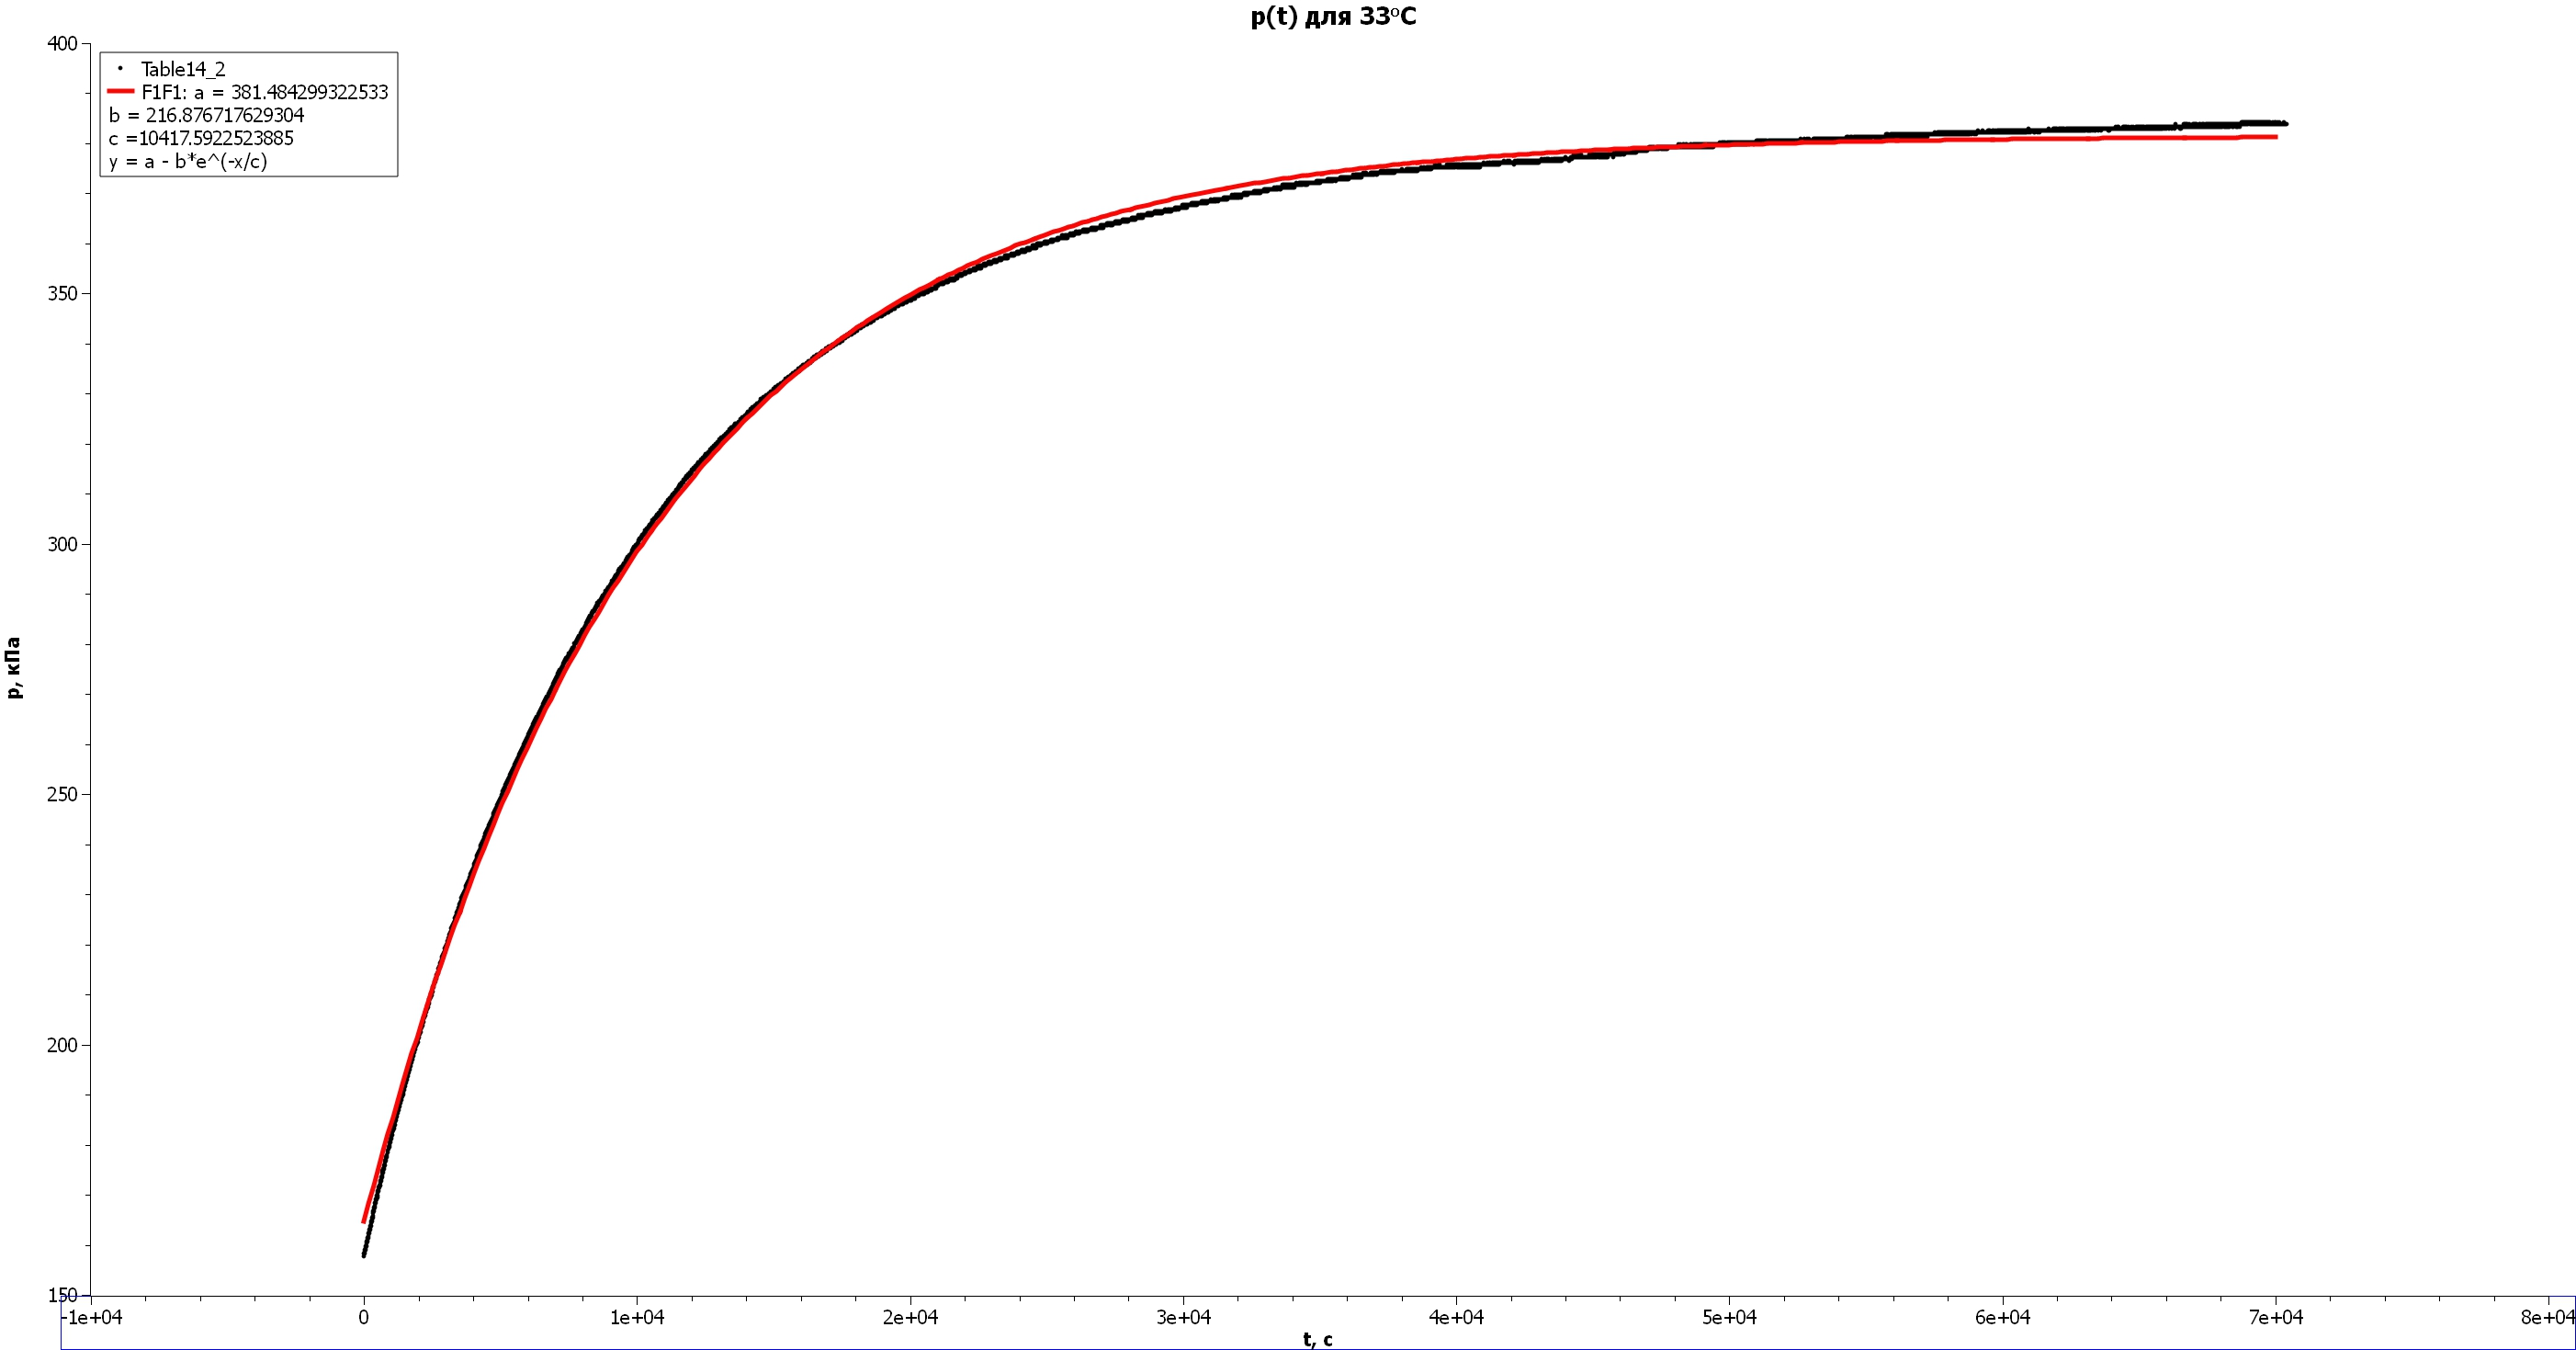
\includegraphics[scale=0.4]{Demo}
\end{flushleft}
Такие измерения були проведены для четырех температур, но даже этого достаточно, чтобы отметить рост скорости выхода газа и максимльного давлени при увеличении температуры, и если построить график зависимости коэффицента С в теоретической формуле от температуры получится такой график.
\begin{flushleft}
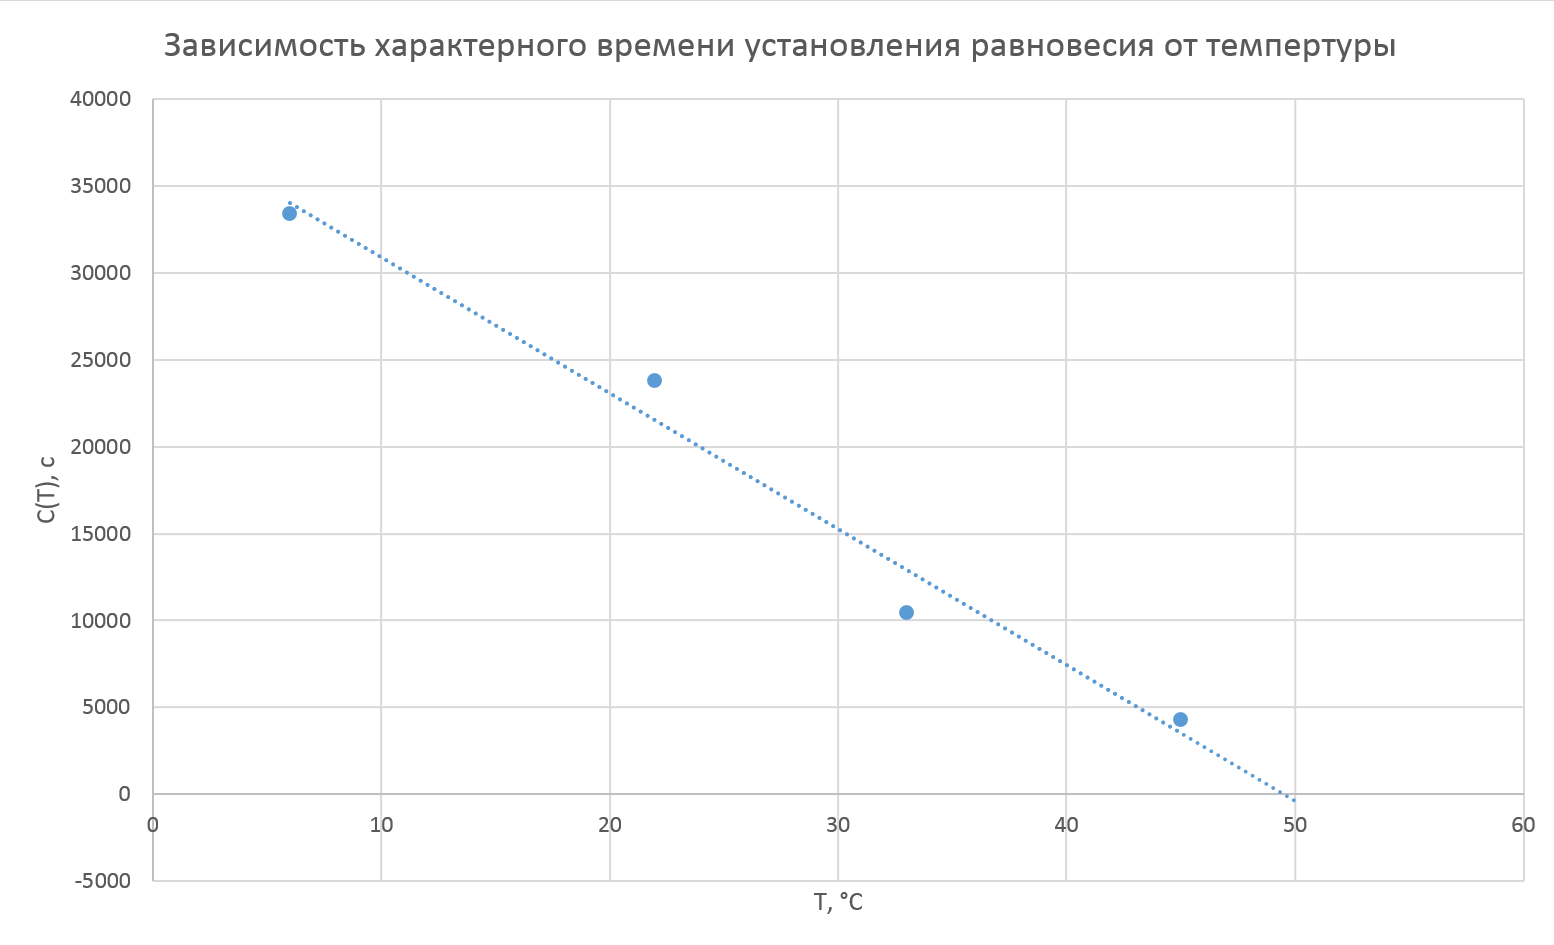
\includegraphics[scale=0.6]{RandomPower}
\end{flushleft}
Сложно по четырем точкам однозначно установить линеен ли этот график, но что-то линейное в нем однозначно есть. Также продление этой зависимости из линейной аппроксимации дает пересечени нуля при температуре около 50 градусов. Физический смысл такой математической неопределенности вида константа делить на ноль в быстром выходе всего газа. При проведении такого эксперимента при 55 градусах пластиковая бутылка раздулась и потеряла формув нижней части образовав там новую выпуклость. При дальнейшем повышении температуры до 80 градусов удалось даже добиться повреждения целосности бутылки силами давления газа внутри.
\begin{flushleft}
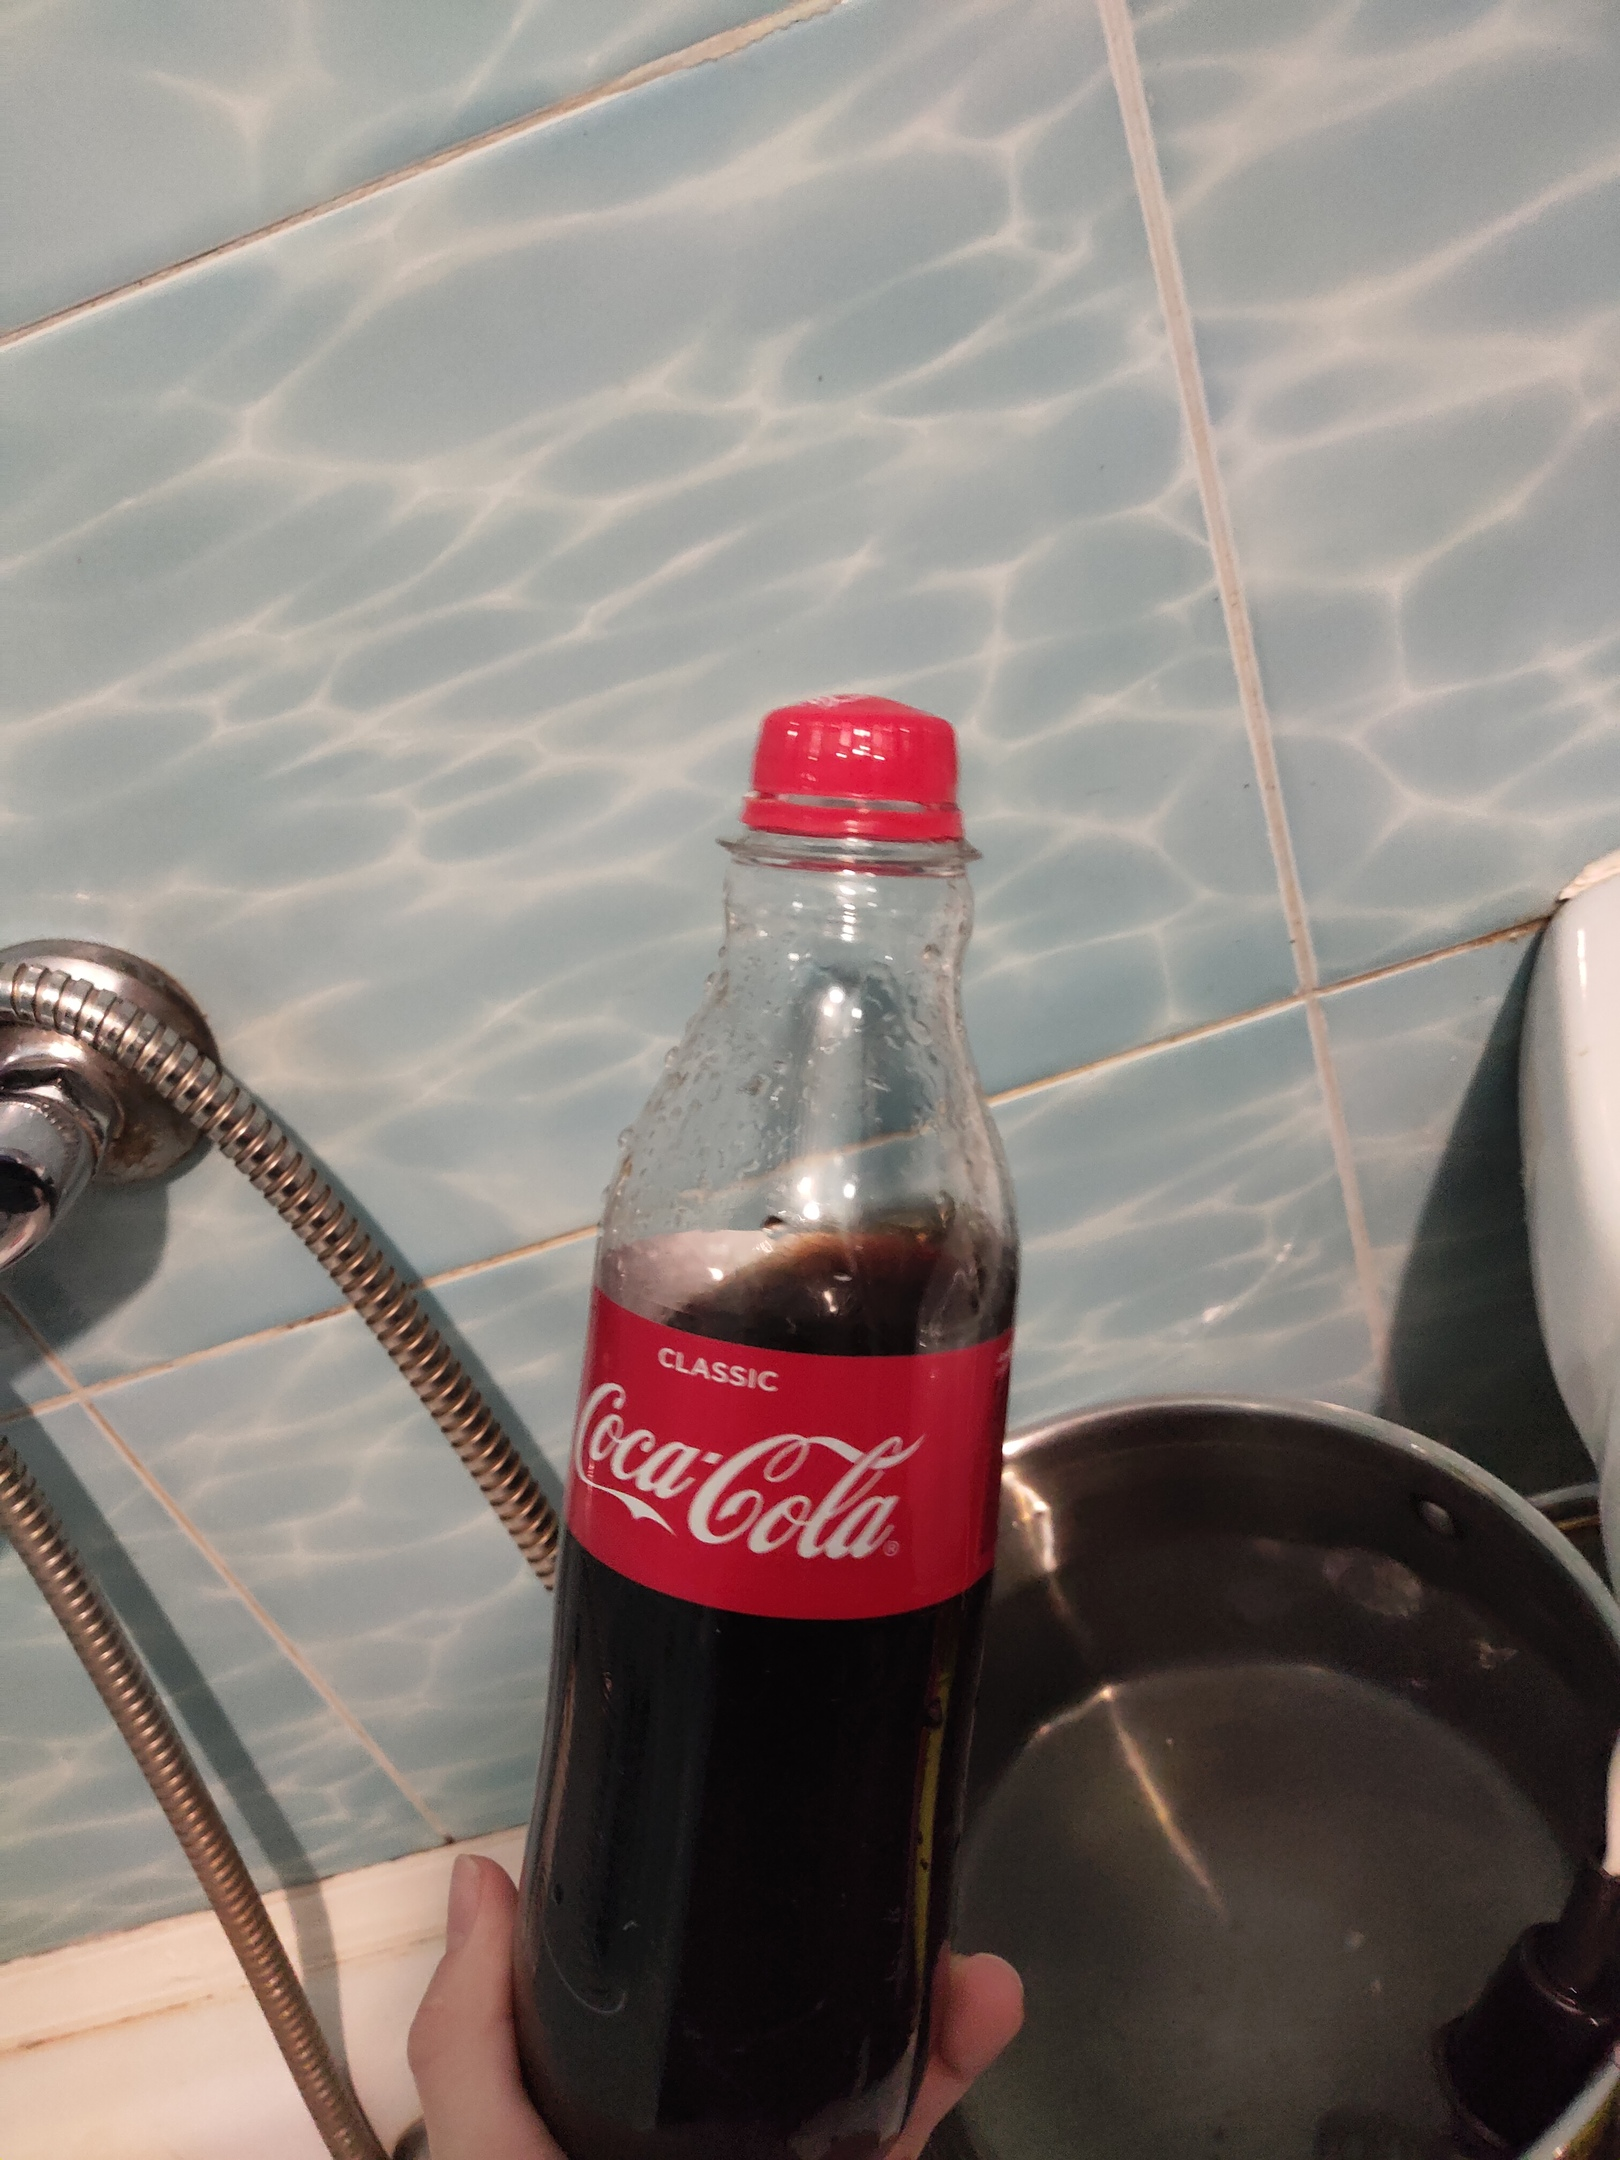
\includegraphics[scale=0.2]{Boom}
\end{flushleft}

С помощью прибора измеряющего объем вышедшего газа потенциально можно найти зависимость скорости выхода газа из раствора в зависимости от концентрации угольной кислоты, преобразовав зависимость объема от времени, но происходит это все очень долго и у занятых учеников ФТШ разумеется не нашлось столько времени, для того чтобы сидеть перед мензуркой и записывать ее показания, но в теории можно автоматизировать и этот процесс. Положив в мензурку яркий попловок и снимая на видео процесс с помощью даже существующей программы можно автоматически получить из такого видео зависимость координаты поплавка от времени, а значит и зависимость объема от времени. У нас не редставлена реализация такого плана по причине нерешенности проблемы с длительной записью видео.

\section{Вывод}




\end{document}
